\documentclass[10pt,a4paper,oneside]{scrreprt}
\usepackage{mystyle}

\begin{document}

\newcommand{\subtitlename}{Master's Thesis}
\newcommand{\titlename}{Refactoring for Scala}

\begin{titlepage}
 
\begin{center}
 
\textsc{\Large University of Applied Sciences Rapperswil}
 
\textsc{\subtitlename}

\rule{0.83\textwidth}{0.4pt}

\vspace{0.2cm}

\normalsize{Spring Semester 2010}

\vspace*{\fill}
 
\Huge{\textit{\titlename}}

\vspace*{\fill}
\vspace{\baselineskip}

\normalsize{\src{scala.ifs.hsr.ch}}

\rule{0.83\textwidth}{0.4pt}
\vskip0.35cm
\begin{minipage}{0.4\textwidth}
\begin{flushleft} \large
\textsc{Author}\\
Mirko Stocker
\end{flushleft}
\end{minipage}
\begin{minipage}{0.4\textwidth}
\begin{flushright} \large
\textsc{Supervisor} \\
Prof. Peter Sommerlad
\end{flushright}
\end{minipage}
 
\end{center}
 
\end{titlepage}


\chapter*{Abstract}

\pagenumbering{roman}

This thesis..


\chapter*{Management Summary}

This documentation 

\newpage

\setcounter{tocdepth}{2}

\tableofcontents

\newpage

\pagenumbering{arabic}

\chapter{Introduction}
\section{Problem Outline}
\section{Thesis Goals}

\chapter{Refactoring Library}

describes the three main modules of the refactoring library.

\section{Overview}

an introduction, mention the basic concepts, also say that trees have to keep their positions if the source code should be regenerated.

\section{Analysis} \label{section:analysis}

An import step in each refactoring is to analyze the current program. For example, when doing a Rename refactoring, we need to resolve all references to the renamed name. A more complex example is Extract Method, where we need to perform data-flow analysis to determine the parameters and return values of the extracted method.

IDEs also analyze the program code in a similar way to make the life of the programmer easier: finding the declaration of a variable or listing all subtypes of a class are common operations.

Our analyses heavily depend on the Scala compiler's AST and all the information it provides through the program's symbols. For example, each symbol has an owner that can be used to navigate the logical structure of the program. There are also almost one hundred \src{isXY} methods defined on the \src{Symbol} class that can be used to query information:

\begin{lstlisting}
abstract class Symbol {
  %\ldots%
  def isAnonymousClass: Boolean
  def isConstructor: Boolean
  def isGetter: Boolean
  def isLocal: Boolean
  def isSubClass(that: Symbol): Boolean
  %\ldots%
}
\end{lstlisting}

All the trees that inherit from the \src{SymTree} trait provide a symbol instance, where \src{DefTrees} usually introduce a new symbol and \src{RefTrees} reference a symbol from a \src{DefTree}. The following illustration shows how symbols are related (not all symbols are colored, for example, the built in types have a symbol as well):

\begin{lstlisting}
trait %\bluebox{SuperClass}% {
  def %\greenbox{strlen}%(%\redbox{str}%: String) = %\redbox{str}%.length
  def %\lgreenbox{abstractMethod}%: Int
}

class %\yellowbox{SubClass}% extends %\bluebox{SuperClass}% {
  def %\greybox{abstractMethod}% = 1 + %\greenbox{strlen}%("1")
}
\end{lstlisting}

Note that the two \src{abstractMethod} symbols are not the same, but there are other means to find overriden and implemented methods in subclasses, as we shall see later.

While the trees can have a reference to a symbol, the converse is not true: symbols do not know about the trees they are related to. But for refactoring, this information is crucial. This is why the refactoring library contains the means to build an index of symbols and corresponding trees.

\subsection{Refactoring Index Interface}

Building an index over a whole project can be expensive, so ideally, the IDE would maintain the index and pass it to the refactoring library when need, in the same way that the library does not compile the source files itself but gets the ASTs directly from the IDE.

The interface that needs to be implemented and is used by the refactorings to query the index looks as follows:

\begin{lstlisting}
trait IndexLookup {
  /**
    * Returns all defined symbols, i.e. symbols of DefTrees.
    * */
  def allDefinedSymbols(): List[global.Symbol]
  
  /**
    * Returns all symbols that are part of the index, either referenced or defined.
    * */
  def allSymbols(): List[global.Symbol]    
  
  /**
    * For a given Symbol, tries to find the tree that declares it.
    * */
  def declaration(s: global.Symbol): Option[global.DefTree]
  /**
    * For a given Symbol, returns all trees that contain a reference to it.
    * */
  def references(s: global.Symbol): List[global.Tree]
  
  /**
    * For a given Symbol, returns all trees that reference or declare the Symbol.
    * */
  def occurences(s: global.Symbol): List[global.Tree]
}
\end{lstlisting}

The library also contains a default implementation that can be used. 

\subsection{Default Index Implementation}

As mentioned previously, building an index can be expensive: whenever a compilation unit in the program changes, references to the symbols from other compilation units can change, and also the other way around. Because of this, it is hard to maintain one monolithic index.

The provided implementation comprises several parts:

\begin{description}
 \item[CompilationUnitIndex] One index per compilation unit that holds the references and declarations of just this part of the program.. This structure can be rebuilt everytime a compilation unit changes. Rebuilding it traverses the whole tree once and stores mappings from symbols to \src{RefTrees} and \src{DefTrees}.
 \item[GlobalIndex] An implementation of the \src{IndexLokup} trait that ties together any number of these per compilation unit indices, but is completely stateless itself.
\end{description}

Whenever a compilation unit changes, one \src{CompilationUnitIndex} needs to be rebuilt and combined with the already existing ones into a new \src{GlobalIndex}.

\subsection{Resolving References}

Resolving the declaration tree of a symbol is an inexpensive lookup, finding all references causes more work. The process of finding all references is done in two steps: first, the symbol is \textit{expanded} and second all references to these expanded symbols are collected. What do we mean by expanding a symbol? Consider the example of the colored symbols we mentioned at the beginning of Section \ref{section:analysis}. The implementing method uses a differen symbol than the abstract declared method. But when we want to find references, we need all references to both symbols. The same is true for getters and setters: renaming a class parameter also needs to rename all useages of getters and setters. To do this, the index implementation uses so called \src{SymbolExpanders}:

\begin{lstlisting}
trait SymbolExpander {
  this: IndexLookup =>
  def expand(s: Symbol): List[Symbol] = List(s)
}
\end{lstlisting}

The \src{SymbolExpander} is used as a stackable trait (XXX ref) and implemented in the following variations:





An example of a finding references to a method.




\section{Transformation}

At the heart of every refactoring lies a \textit{transformation} that takes the current program in its abstract syntax tree form and transforms it into its refactored form. Such a transformation can be as simple as changing names -- think of the Rename refactoring -- or restructure large parts of the AST as in an Extract or Move refactoring. 

Often, a larger refactoring comprises many smaller transformations. An illustrative example is the Extract Method refactoring, which can be assembled from three basic transformations:

\begin{description}
 \item[Create Method] to introduce a new (empty) method.
 \item[Copy Statements] to copy the selected statements into the newly created method.
 \item[Replace Statements] to replace the original statements that have been copied to the new method with a call to it.
\end{description}

The \textit{replace} transformation itself is again a combination of two even more fundamental transformations: \textit{insert} and \textit{delete}. Once we have our Extract Method transformation, it can then again be combined with other transformations -- for example into an Extract Class refactoring. It should be clear from this that the key to a reusable refactoring library lies in the composability of its transformations. 

Conceptually, chaining simple transformations to build more powerful ones follows the Unix pipes philosophy. The design of this implementation was inspired by the Stratego program transformation tool-set (referenz) and the Kiama language processing library (referenz). Functional programming also uses the term \textit{combinator} to denote functions that can be combined and yield new functions of the same kind. An example of this are parser combinators (referenz), which are part of the Scala standard library.

In contrast to unix pipes that operate on their input line by line, performing transformations on a tree datastructure adds an additional dimension. When transforming trees, we are also concerned with questions on how we want to traverse the tree -- i.e. pre-order or post-order -- and to which children a transformation should be applied. The presented implementation handles all these concerns in a uniform way.

In the remainder of this section, we will develop the basics of our transformation combinators and show examples of their usage.

\subsection{Transformations}

A refactoring transformation is essentially a function that transforms a tree into an other tree. But because most transformations do not apply to all kinds of possible trees, we model a transformation as a function of type $Tree\Rightarrow Option[Tree]$, making use of Scala's \src{Option} monad to indicate inability to transform. In the actual implementation, the transformations are implemented generically as a \src{Transformation[A,~B]} that extend \src{A~$\Rightarrow$~Option[B]}:

\begin{lstlisting}
abstract class Transformation[A, B] extends (A %$\Rightarrow$% Option[B]) {
  self %$\Rightarrow$%

  def apply(in: A): Option[B]
%\ldots%
}
\end{lstlisting}

The explicit self type annotation\footnote{In this case, think of the self type annotation as an alias for \src{this} that can be used in the body of the class.} will be used later in the implementation of the combinators. Note that all transformations are implemented polymorphic, but to make the explanations more clear, we will assume that they are used to transform trees.

Transformations can be created from partial functions using the \src{transformation} convenience function. As an example, we create a transformation that reverses the order of a class, trait, or object's member definitions and apply it to a given template instance.

\begin{lstlisting}
def transformation[A, B](f: PartialFunction[A, B]) = new Transformation[A, B] {
  def apply(t: A): Option[B] = f lift t
}

val reverseTemplateMembers = transformation[Tree, Tree] {
  case t: Template %$\Rightarrow$% t copy (body = t.body.reverse)
}

val result: Option[Tree] = reverseTemplateMembers(template)
\end{lstlisting}

Now that we have a way to create single transformations, we need to be able to combine them. To do this in various ways, we introduce several combinators. We use a notational shortcut to denote transformations: $A \overset{t}{_\rightarrow} [B]$ is a \src{Transformation [A, B]}.

There also exist two basic transformations, one that always succeeds, returning its input unchanged, and one that always fails, independent of its input. Depending on the context, the alias \src{id} for \src{succeed} might be a better fit and is provided as well.

\begin{lstlisting}
def succeed[A] = new Transformation[A, A] {
  def apply(a: A): Option[A] = Some(a)
}

def id[A] = success[A]

def fail[A] = new Transformation[A, A] {
  def apply(a: A): Option[A] = None
}
\end{lstlisting}

\subsection{Combinators}

There are several existing combinators already implemented in the library. On the right side of each paragraph, the symbolic or alphanumeric name and type of the transformation is shown.

\paragraph{Sequence} \hfill \lstinline{&>: } $(A \overset{t}{\rightarrow} [B]) \Rightarrow (B \overset{t}{\rightarrow} [C]) \Rightarrow (A \overset{t}{\rightarrow} [C])$

\vspace{7pt} Combines two transformations so that the second one is only applied when the first one succeeded. The result of the first transformation is passed into the second one. This is implemented as the \src{andThen} method -- or alternatively with the \src{\&>} operator -- on \src{Transformation}, which takes the second transformation as a by-name parameter:

\begin{lstlisting}
abstract class Transformation[A, B] extends (A %$\Rightarrow$% Option[B]) {
  self %$\Rightarrow$%

  def apply(in: A): Option[B]

  def andThen[C](t: %$\Rightarrow$% Transformation[B, C]) = new Transformation[A, C] {
    def apply(a: A): Option[C] = {
      self(a) flatMap t
    }
  }
  def &>[C](t: %$\Rightarrow$% Transformation[B, C]) = andThen(t)
%\ldots%
\end{lstlisting}


\paragraph{Alternative} \hfill \lstinline{|>: } $(A \overset{t}{\rightarrow} [B]) \Rightarrow (A \overset{t}{\rightarrow} [B]) \Rightarrow (A \overset{t}{\rightarrow} [B])$

\vspace{7pt} Combines two transformations so that the second one is only applied in case the first one fails. The implementation is directly based on the underlying \src{Option} type in the \src{orElse} method on \src{Transformation} and also has an operator alias:

\begin{lstlisting}
abstract class Transformation[A, B] extends (A %$\Rightarrow$% Option[B]) {
  self %$\Rightarrow$%

  def apply(in: A): Option[B]

  def orElse(t: %$\Rightarrow$% Transformation[A, B]) = new Transformation[A, B] {
    def apply(a: A): Option[B] = {
      self(a) orElse t(a)
    }
  }
  def |>(t: %$\Rightarrow$% Transformation[A, B]) = orElse(t)
%\ldots%
\end{lstlisting}

With these two combinators, we are already able to represent conditional transformations. For example, given a transformation \src{isClass} that acts as a predicate, and two transformations \src{a} and \src{b} that represent the two possible branches the transformation can take, we can combine them into a new transformation \src{isClass \&> a |> b} that executes the \src{a} transformation if the \src{isClass} transformation succeeds or \src{b} if either \src{isClass} or \src{a} fails.

Note that due to Scala's precedence rules, the \src{|>} combinator has a lower precedence than \src{\&>}.

\paragraph{Predicate} \hfill \lstinline{predicate: } $(A \overset{?}{\rightarrow} Boolean) \Rightarrow (A \overset{t}{\rightarrow} [A])$

\vspace{7pt} As we have seen, transformations can be used as predicates. We often want to construct a predicate from a function that returns a boolean value. This can be done with the \src{predicate} function which create a transformation from a partial function.

\begin{lstlisting}
def predicate[A](f: %$\Rightarrow$% PartialFunction[A, Boolean]) = new Transformation[A, A] {
  def apply(a: A): Option[A] = if (f.isDefinedAt(a) && f(a)) Some(a) else None
}
\end{lstlisting}

\paragraph{Not} \hfill \lstinline{!: } $(A \overset{t}{\rightarrow} [A]) \Rightarrow (A \overset{t}{\rightarrow} [A])$

\vspace{7pt} A combinator that inverts a transformation. Given a transformation that succeeds, then \src{not} will fail. Should the given transformation fail, then \src{not} returns the original input unchanged. This behavior is useful for transformations that act as predicates; \src{not} can be implemented using the \src{fail} and \src{id} transformations as follows.

\begin{lstlisting}
def not[A](t: %$\Rightarrow$% Transformation[A, A]) = t &> fail |> succeed
\end{lstlisting}

Now that we have several means to specify and combine our transformations, we also need a way to apply them to a whole AST, instead of just single tree nodes. For this, there exist several traversal strategies.

\subsection{Traversal}

Applying a transformation to a single tree element is not difficult, but once we want to traverse the whole AST, we need a way to apply a transformation to all children of a tree node and to construct a new tree from the result of the transformation operation. Note that traversal strategies are also just transformations that can again be combined.

\paragraph{All Children} \hfill  $allChildren: (A \overset{t}{\rightarrow} [B]) \Rightarrow (A \overset{t}{\rightarrow} [B])$

\vspace{7pt} Takes a transformation and creates a new one that applies the given transformation to all children, returning a single tree. Because there is no generic way to get all children and construct a new tree, we constrain the type parameter \src{A} to be convertible to $(A \Rightarrow B) \Rightarrow B$. This means that the user of the generic transformation has to pass us its children and create a new tree. When a child cannot be transformed, \src{allChildren} immediately aborts and returns \src{None}.

\begin{lstlisting}
def allChildren[A <%\%% (A %$\Rightarrow$% B) %$\Rightarrow$% B, B](t: %$\Rightarrow$% Transformation[A, B]) = new Transformation[A, B] {
  def apply(a: A): Option[B] = {
    Some(a(child %$\Rightarrow$% t(child) getOrElse (return None)))
  }
}
\end{lstlisting}

(\src{X <\% Y} is called a \textit{view bound} and demands that there exists an implicit conversion from type \src{X} to \src{Y}. This is less constrictive than \src{X <: Y}, where \src{X} has to be a subtype of \src{Y}. In our case, we can then treat \src{a} as if it were of type \src{(A $\Rightarrow$ B) $\Rightarrow$ B}. This allows us to apply the transformation to the children of \src{a}.)

\paragraph{Matching Children} \hfill $matchingChildren: (A \overset{t}{\rightarrow} [A]) \Rightarrow (A \overset{t}{\rightarrow} [A])$

\vspace{7pt} The \src{allChildren} traversal only succeeds when the transformation can be applied to all children. If children that cannot be transformed should simply be kept and passed to the new tree unchanged, we can use the \src{matchingChildren} transformation.

\begin{lstlisting}
def matchingChildren[A <%\%% (A %$\Rightarrow$% A) %$\Rightarrow$% A](t: Transformation[A, A]) = allChildren(t |> id[A])
\end{lstlisting}

Using the \src{id} transformation, we retain the original tree should the transformation not be applicable. A consequence of this is that the transformation needs to be done between the same types.

%\paragraph{Once} \hfill \lstinline{once: } $(A \overset{t}{\rightarrow} [A]) \Rightarrow (A \overset{t}{\rightarrow} [A])$

%\vspace{7pt} Applies a transformation and stops on the first successful application... not yet implemented.

The next step after being able to apply a transformation to a tree or all of its children is to expand this to the AST as a whole. We can distinguish between two fundamental ways of transforming a tree: either in a pre-order or post-order fashion.

\paragraph{Pre-Order} \hfill $\downarrow: (A \overset{t}{\rightarrow} [A]) \Rightarrow (A \overset{t}{\rightarrow} [A])$

\vspace{7pt} Pre-order application of a transformation applies the transformation to the parent first and then descends into its children. The consequence is that at the time a tree gets transformed, its children are still in their original, untransformed state.

\begin{lstlisting}
  def %$\downarrow$ \hspace{19pt} %      [A <%\%% (A %$\Rightarrow$% A) %$\Rightarrow$% A](t: Transformation[A, A]) = t &> allChildren(%$\downarrow$%(t))
  def preorder[A <%\%% (A %$\Rightarrow$% A) %$\Rightarrow$% A](t: Transformation[A, A]) = %$\downarrow$%(t)
\end{lstlisting}

Using a pre-order transformation has the benefit that trees are always in their original state when they are transformed, this can be used when the trees need to be compared for equality. A disadvantage is that a transformation can diverge when it modifies a tree so that it again applies to one of its new children. For example, applying the following transformation to a tree results in a stack overflow when applied with pre-order traversal:

\begin{lstlisting}
transformation[Tree, Tree] {
  case block @ Block(stats, _) => block copy (stats = block :: stats)
}
\end{lstlisting}

This will not happen when the transformation is applied using post-order traversal.

\paragraph{Post-Order} \hfill $\uparrow: (A \overset{t}{\rightarrow} [A]) \Rightarrow (A \overset{t}{\rightarrow} [A])$

\vspace{7pt} Bottom-up application first descends into the children of a tree and processes the parent after the children. Thus once a tree gets transformed, its children have already been transformed.

\begin{lstlisting}
  def %$\uparrow$ \hspace{27pt} %      [A <%\%% (A %$\Rightarrow$% A) %$\Rightarrow$% A](t: Transformation[A, A]) = allChildren(%$\uparrow$%(t)) &> t
  def postorder [A <%\%% (A %$\Rightarrow$% A) %$\Rightarrow$% A](t: Transformation[A, A]) = %$\uparrow$%(t)
\end{lstlisting}

Combining all these transformations with combinators and traversal strategies allows us to describe transformations in a very concise way.

\figref{figure:traversal_mode} illustrates the difference between the two traversal modes.

\begin{figure}
 \centering
 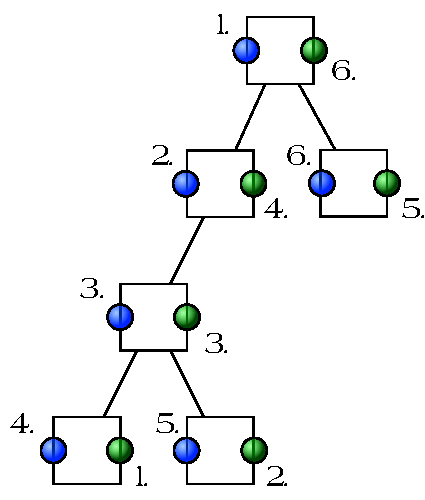
\includegraphics[width=0.4\linewidth]{traversal_mode.pdf}
 \caption{An illustration of the pre- and post-order traversal strategies: the blue points show the order in which the tree gets transformed in pre-order traversal, and the green ones illustrate the post-order traversal. Instead of pre- and post-order, we can also think of the transformations being applied top-down or bottom-up, hence the $\downarrow$ and $\uparrow$ aliases.}
 \label{figure:traversal_mode}
\end{figure}

As a first example, let us write and use a transformation that replaces all trees in the AST which do not have a range position with the \src{EmptyTree}.

\begin{lstlisting}
val tree: Tree = %\ldots%

val emptyTree = transformation[Tree, Tree] {
  case t if t.pos.isRange => t
  case _ => EmptyTree
}

preorder(allChildren(emptyTree)) apply tree
\end{lstlisting}

Preorder traversal already applies the transformation to all children, so we can simplify this to:

\begin{lstlisting}
preorder(emptyTree) apply tree
\end{lstlisting}

Of course, this is not the only way to achieve this, here is a variation that separates the testing for the range position into a predicate and uses a simple transformation to replace the tree. If the tree has a range position, it is not transformed (remember that the \src{id} transformation simply returns its argument unchanged). In case the predicate fails, the tree is replaced.

\begin{lstlisting}
val hasRangePosition = predicate((t: Tree) => t.pos.isRange)

val emptyTree = transformation[Tree, Tree] {
  case _ => EmptyTree
}

preorder(hasRangePosition &> id[Tree] |> emptyTree) apply tree
\end{lstlisting}

Using the \src{not} combinator, we can swap the two actions:

\begin{lstlisting}
preorder(not(hasRangePosition) &> emptyTree |> id[Tree]) apply tree
\end{lstlisting}

To get rid of the \src{id} transformation, we can use a different traversal strategy for the children:

\begin{lstlisting}
preorder(matchingChildren(not(hasRangePosition) &> emptyTree)) apply tree
\end{lstlisting}

More examples can be found in Section \vref{subsection:tree-transformations}.

\subsection{Creating Trees}

Most refactorings do not just reuse existing trees but also have to create new ones. The Scala compiler already contains several facilities to create new trees: the trait \src{scala.tools.nsc.ast.Trees} contains many methods that create AST trees and there's even a DSL in \src{scala.tools.nsc.ast.TreeDSL} whose ``goal is that the code generating code should look a lot like the code it generates''.

An example from \src{Trees} shows how many methods there are to create method definitions (this code has obviously been written before Scala had default arguments):

\begin{lstlisting}
def DefDef(sym: Symbol, mods: Modifiers, vparamss: List[List[ValDef]], rhs: Tree): DefDef

def DefDef(sym: Symbol, vparamss: List[List[ValDef]], rhs: Tree): DefDef
  
def DefDef(sym: Symbol, mods: Modifiers, rhs: Tree): DefDef

def DefDef(sym: Symbol, rhs: Tree): DefDef

def DefDef(sym: Symbol, rhs: List[List[Symbol]] => Tree): DefDef
\end{lstlisting}

Using the TreeDSL allows one to write very concise code. The following listing creates the AST for the code that checks whether \src{tree} is null.

\begin{lstlisting}
IF (tree MEMBER_== NULL) THEN %\ldots% ELSE %\ldots%
\end{lstlisting}

Unfortunately, all these tree construction helpers are problematic for us: they can change the position of the trees, which we have to avoid when we want to retain the source code layout. For this reason, the refactorings do not make use of these facilities but simply create the trees from scratch. There are some helper methods in \src{transformation.TreeFactory} which take care of constructing trees that are needed by the currently implemented refactorings:

\begin{lstlisting}
def mkRenamedSymTree(t: SymTree, name: String): SymTree

def mkReturn(s: List[Symbol]): Tree

def mkValDef(name: String, rhs: Tree): ValDef

def mkCallDefDef(name: String, arguments: List[List[Symbol]], 
  returns: List[Symbol]): Tree

def mkDefDef(mods: Modifiers, name: String, 
  parameters: List[List[Symbol]], body: List[Tree]): DefDef

def mkBlock(trees: List[Tree]): Block
\end{lstlisting}

Now that we have seen how trees can be transformed and how new trees can be generated, we are ready for a larger example.

\subsection{Tree Transformations}\label{subsection:tree-transformations}

For the usage in the refactoring, the \src{TreeTransformations} trait implements the traversal for Scala's AST and provides some definitions that make writing transformations more concise:

\begin{lstlisting}
def transform(f: PartialFunction[Tree, Tree]) = transformation(f)
  
def filter(f: %$\Rightarrow$% PartialFunction[Tree, Boolean]) = predicate(f)
\end{lstlisting}

Let us now take a look at a larger example: Extract Method. At the beginning of this section, we looked at the different transformations that occur during the refactoring: Insert a new method with the extracted statements and replace them with a call to this new method. This can be achieved with the following transformations:

\begin{lstlisting}
val replaceBlockOfStatements = transform {
  case block @ BlockExtractor(stats) => {
    mkBlock(stats.replaceSequence(selectedTrees, callExtractedMethod))
  }
}

val replaceSingleExpression = transform {
    case t if t == selectedTree => callExtractedMethod
}

val replace = topdown {
  matchingChildren {
    if(extractSingleTree)
      replaceSingleExpression
    else
      replaceBlockOfStatements
  }
}

val insertExtractedMethod = transform {
  case tpl @ Template(_, _, body) => 
    tpl copy (body = body ::: extractedMethod :: Nil) setPos tpl.pos
}
\end{lstlisting}

A remark on the call to \src{setPos tpl.pos} in \src{insertExtractedMethod}: Because the structure of a tree is immutable, we cannot change a tree in-place, even though we often want to do this. The source regeneration uses the position information of the trees to determine whether a tree's existing source code can be reused. So if we want a tree to appear modified in-place, we simply assign it the position of the original tree. Note that this does only work if the two trees are of the same type.

Next we need two filters that find the enclosing class' template and the method we extract from:

\begin{lstlisting}
val findTemplate = filter {
  case Template(_, _, body) => body exists (_ == selectedMethod)
}

val findMethod = filter {
  case d: DefDef => d == selectedMethod
}
\end{lstlisting}

Now we can combine these to assemble a new transformation that performs the following steps:

\begin{enumerate}
 \item Traverse the tree until the selected template is found, the one that contains \src{selectedMethod}.
 \item Once we found the template, start the following two transformations:
  \begin{enumerate}
        \item Find the method we extract from and apply the \src{replace} transformation on it.
        \item Insert the new method in the class template.
       \end{enumerate}
\end{enumerate}

%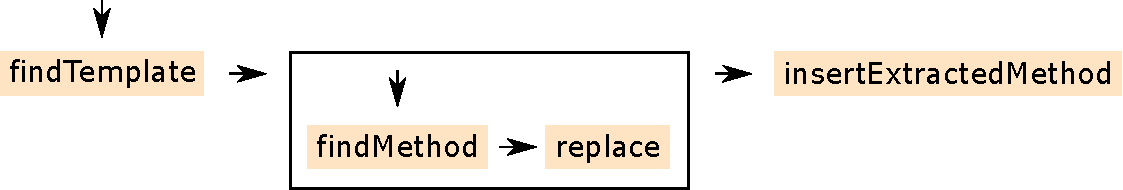
\includegraphics[width=\linewidth]{extract_method_transformation.pdf}

All these steps can be expressed with a simple transformation:

\begin{lstlisting}
val extractMethod = topdown {
  matchingChildren {
    findTemplate &> 
    topdown {
      matchingChildren {
	findMethod &> replace
      }
    } &> 
    insertExtractedMethod
  }
}
\end{lstlisting}

\section{Code Generation}

Once our abstract syntax tree has been refactored, we need to convert it back into its textual source code representation. This process comprises two main steps: the \textit{detection of modifications} to minimize the amount of code that is regenerated and the actual \textit{source generation}.

The first step is necessary because we -- in contrast to many other refactoring implementations -- do not keep track of modifications to the AST while they are happening but reconstruct this information afterwards. This allows us to keep the transformations simpler but consequently makes the code generation more complex. This tradeoff is worthwile because we intend the library to be reused and the transformations to be implemented by third parties.

The AST after the refactoring may contain several kinds of modifications. Trees can be moved around, deleted and new trees can be introduced. From the transformations we know that trees that are moved around keep their original position information, and newly created trees have a \src{NoPosition} attribute per default. This allows us to detect changes and can later be used during source generation to preserve the layout of already existing trees. 

\subsection{Modification Detection}

The primary goal of a fine-grained modification detection is to reduce the amount of trees that are regenerated. The source generation is invoked with a list of trees from various files that all can have an arbitrary number of changed children:

\begin{lstlisting}
def createChanges(ts: List[Tree]): Iterable[Change]
\end{lstlisting}

Modification detection performs the following three steps on the input trees:

\begin{enumerate}
 \item Group all changed trees by their file.
 \item Find the top-level changed trees for each file.
 \item Detect the change-set per top-level tree.
\end{enumerate}

Top-level trees are trees that are ancestors of other changed trees. For example, the following graph shows an AST with some changed trees in green and blue:

\begin{center}
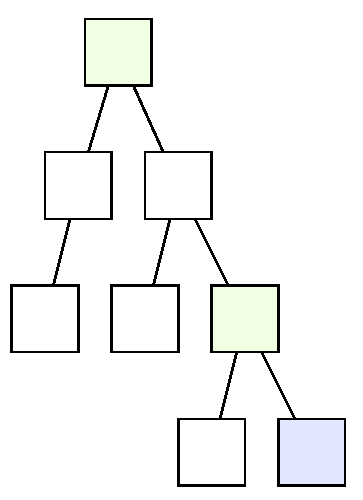
\includegraphics[width=0.2\linewidth]{ast_with_changes.pdf}
\end{center}

The \src{createChanges} method is invoked with the two green trees, but the blue tree has also been modified by a transformation.

Now if we were to generate two changes from the two green trees, we would get a problem when applying the changes because they overlap each other. The two changes would either overwrite each other or, in the case of Eclipse's Language Toolkit, yield an error. Therefore the second step of the modification detection is to find those trees that contain other changed trees. In the AST above, this would be the root node.

The third step then traverses these top-level trees and finds all changes as well as the trees that lie between changed trees, here marked in blue:

\begin{center}
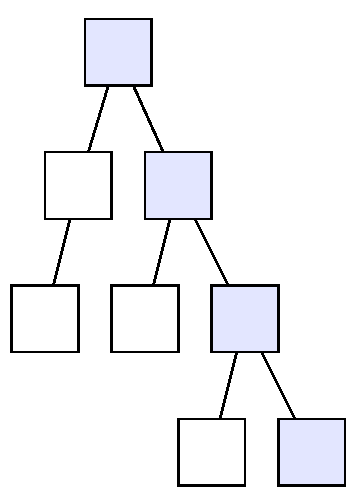
\includegraphics[width=0.2\linewidth]{ast_with_changeset.pdf}
\end{center}

This set of trees is the minimal number of trees that need to be regenerated. Trees that are not contained in the set can be kept as they are to improve the performance. \figref{figure:ast_with_changes_large} shows a larger example of the process.

\begin{figure}
 \centering
 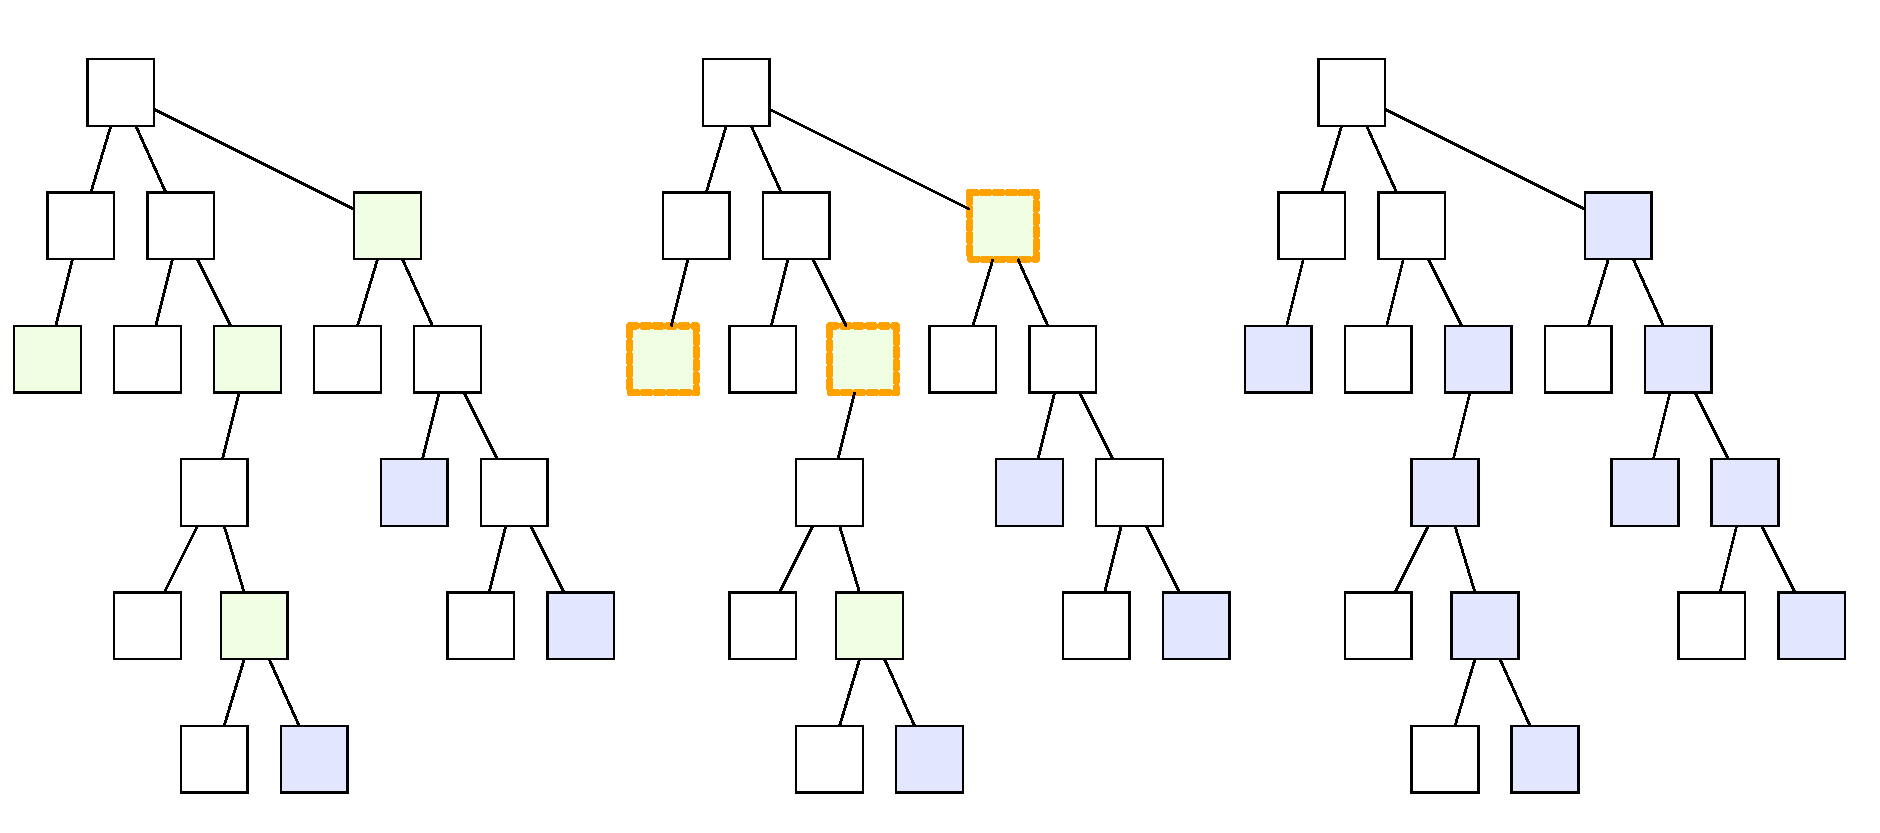
\includegraphics[width=\linewidth]{./ast_with_changes_large.pdf}
 \caption{An example of how the change set is built: the left AST shows in green the list of all trees that should be regenerated, but the blue trees have changed as well. In the middle graph, we see the trees that were identified as top-level trees. The rightmost AST shows all trees that need to be regenerated.}
 \label{figure:ast_with_changes_large}
\end{figure}

Once we have identifier all top-level tree changes, we start generating source code for them. 

\subsection{Source Code Generation}

The AST does by its very nature not contain all the information that is necessary to fully reconstruct its original textual representation. Also, syntactic sugar of the programming language is usually not represented in the AST but only available in its generalized form. An example for this are Scala's \src{for} comprehensions. They are equivalent with function calls to \src{map, filter, flatMap,} and \src{foreach}. This means that the two statements in the following listing have the same representation in the AST.

\begin{lstlisting}
val v1 = List(1,2,3) map (i => i * 2)
val v2 = for(i <- List(1,2,3)) yield i * 2
\end{lstlisting}

Other things that are not mentioned explicitly in the AST are parenthesis, commas and many other tokens. In the context of source generation, we will call them layout elements, or just \textit{layout}. 

If we were only interested in a semantically equivalent program, we could simply pretty print the AST to generate the source code. No user of a refactoring tool would accept this, so we need another technique. 

The source code is always available to the refactoring tool, and with the position information on the trees, we have a means to look up the original source code for a tree.

Other refactoring tools (TODO ref) have used various approaches to solve this problem. For some cases -- for example in a rename refactoring -- it might even be acceptable to pretty print the code as long as only very small regions of the program change. This approach can be problematic -- for example with the Extract Method refactoring, where arbitrary large parts of the program are moved around. A tool can handle this situation by cut-and-pasting the body of the extracted method. This is not feasible for us because we need a generic way to handle all kinds of unforseeable changes to the source code.

\subsubsection{Preserving Layout}

Our approach is based on using two different kinds of source printers: one that pretty prints code  and another one that reuses the existing code where possible. The \textit{pretty printer} simply prints the code with a default layout and is used for trees that were introduced during the transformation. The \textit{reusing printer} takes the existing layout with the help of the trees's position information and also makes sure all needed layout elements are present. How this is done will be explained in more detail later.

The source generation algorithm then alternates between these two printers during the code generation process.

Now we just need to know how we can reuse the existing layout. What we need is a way to decide how all these layout elements can be associated to their enclosing trees. If we take a look at the following listing, we can see several occurences of whitespace and other layout, like the three comments and the braces.

\begin{lstlisting}
package p //TODO
// myclass
class MyClass(a: Int /* the int */) {
}
\end{lstlisting}

Because no rules of the programming language dictate how the layout is associated with the other parts of the program, we have to guess how to divide it and associate it with its surrounding trees. Often this can be done by taking the types of the adjacent trees into consideration and then divide the layout according to some rules and regular expressions. 

For example, one rule says that the layout between two enclosing value definitions is split by a comma, or by newline if there is no comma present. So when the values are part of an argument list, they will get comma-separated, and if they are definitions, the layout will be split at the end of the line, so that the first value will get all layout that follows on its line. Comments can be handled with the same rules as well: a comment on a preceding and otherwise empty line is associated with the following tree.

Let us take a look at a concrete example. \figref{figure:ast_with_layout} shows the AST of the previous listing and how the layout elements have been associated with the left and right sides of a tree. Note that the \src{class} and \src{package} keywords are also considered layout, this is because they are not represented in the AST with their own tree and position information.

\begin{figure}
 \centering
 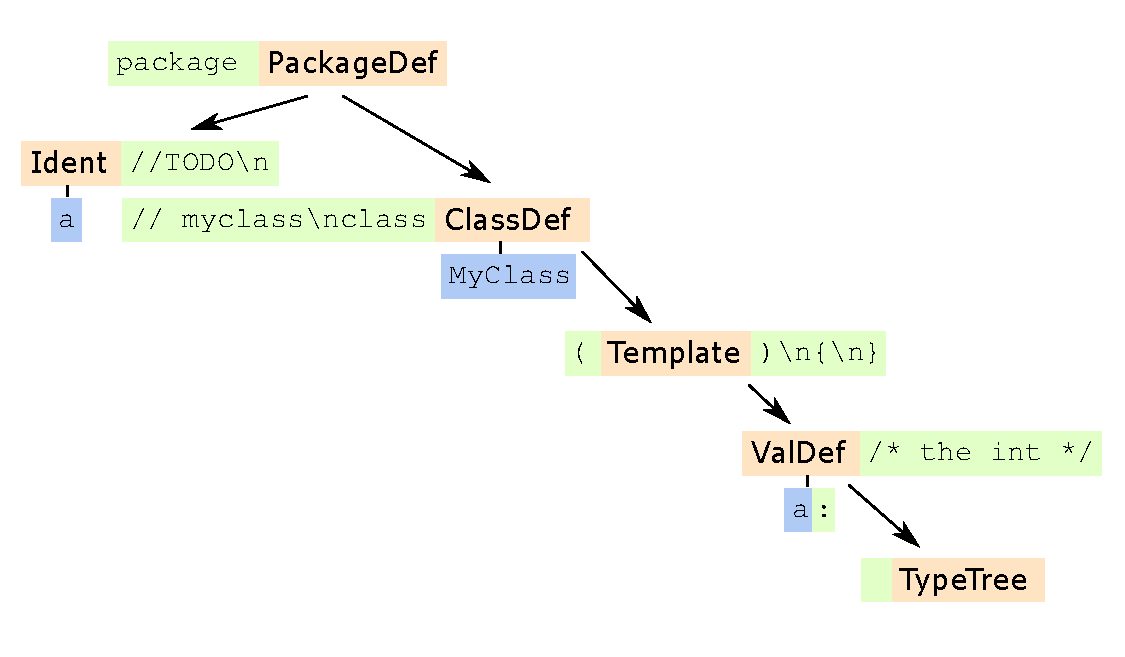
\includegraphics[width=0.8\linewidth]{ast_with_layout.pdf}
 \caption{An example of how layout can be associated with trees: the apricot colored boxes represent the trees and the green ones their associated layout. The blue parts are not real AST nodes but names; they are treated like trees in the source generation.}
 \label{figure:ast_with_layout}
\end{figure}

Once we have identified the layout that belongs to a tree, we can use it during the source generation. For example, it should be clear now that when we would delete the \src{ValDef} parameter in the above AST, then the comment would be removed along with it.

Another issue that concerns both the pretty and the reusing printer is the indentation of the code. When a new statement in a block of other statements is inserted, we want it to have the same indentation as its siblings. For this, the printers also keep track of the currently desired indentation as specified by the parent tree. 

Whether we can reuse existing code or have to invoke the pretty printed needs to be decided for each tree in the AST. This gives us the following definition of the various source printers:

\begin{lstlisting}
trait AbstractPrinter {
  def print(t: Tree, ind: Indentation): Fragment
}

trait PrettyPrinter extends AbstractPrinter {
  def print %\ldots%
}

trait ReusingPrinter extends AbstractPrinter {
  def print %\ldots%
}

trait SourceGen extends PrettyPrinter with ReusingPrinter {
  override def print(t: Tree, i: Indentation): Fragment = {
    if(t.hasExistingCode)
      super[ReusingPrinter].print(t, i)
    else if(t.hasNoCode)
      super[PrettyPrinter].print(t, i)
    else
      EmptyFragment
  }
%\ldots%
\end{lstlisting}

What we have not yet explained is the \src{Fragment} type.

\subsubsection{Fragments and Layout}

The result of a printing operation is not a plain string but an instance of \src{Fragment}. A fragment contains a leading, center, and trailing layout. A layout is simply a wrapper around a string or a part of the source file with some additional helper methods. For example, in \figref{figure:ast_with_layout}, all the apricot and blue colored boxes are fragments and the green ones are instances of \src{Layout}.

The fragments and layouts are created in the printers, where they pattern match on the tree and recursively print the children of a tree. This is an excerpt from the pretty printer:

\begin{lstlisting}
def print(t: Tree, ind: Indentation) = t match {
  case PackageDef(pid, stats) =>
    Layout("package ") ++ 
      printTree(pid, after = newline) ++ 
      printTrees(stats, separator = newline)
%\ldots%
\end{lstlisting}

The \src{++} operation on the layout and the fragments simply concatenate their operands, again yielding a fragment. So far, we could also have just used plain Strings and concatenate them with \src{+}, except that using strings weakens the typesystem because every object can be concatenated to a String using the implicit \src{toString} method.

\subsubsection{Reusing Layout}

The printers also have to take care that all the necessary layout is printed when needed. This can become difficult when layout is reused. Imagine the following scenario: We create a new \src{Block} (a \src{Block} tree wraps a list of other statements) and insert several statements into it. The pretty printer separates each statement in a block with a newline, so the code to pretty print a block could look like this:

\begin{lstlisting}
case Block(stats) =>
  Layout("{"+newline) ++ 
    printTree(stats, separator = newline) ++ 
    Layout(newline+"}")
\end{lstlisting}

This works fine as long as the statements are not reused trees that might already have a leading or trailing newline in their associated layout. If this is the case, we could get too many blank lines between our statements. 

To solve this, the pretty printer could print the block's children one by one and then check if the newline is already present or needs to be inserted. This is tedious to do in every place where a layout element is inserted, so we need a more generic way to handle such cases, and this is where the \src{Requisites} come into play. Instead of specifying the layout directly, the printers simply declare that there needs to be a newline present in the surrounding layout:

\begin{lstlisting}
case Block(stats) =>
  Requisite("{"+newline) ++ 
    printTree(stats, separator = Requisite(newline)) ++ 
    Requisite(newline+"}")
\end{lstlisting}

Now during the concatenation of fragments and layout objects with \src{++}, it is checked whether a certain requisite is already satisfied. The layout is only generated when it is nedeed.

This leads us to the following three interfaces (the \src{++} operators and some other methods have been omitted) that are used to represent the source code in the printers:

\begin{lstlisting}
trait Layout {
  def asText: String
}

trait Requisite {  
  def isRequired(l: Layout, r: Layout): Boolean
  def apply(l: Layout, r: Layout): Layout
}

trait Fragment {
  def leading:  Layout
  def center:   Layout
  def trailing: Layout
  
  def pre: Requisite
  def post: Requisite
  
  def asText: String
}
\end{lstlisting}

(hier muss noch was kommen, aber was? mehr beispiele?)

\subsection{Using the Source Generator}

To users of the code generation, the \src{createChanges} method of the \src{SourceGen} trait creates the change objects from a list of trees by first narrowing down the changed trees and then generating the code for them. The result is a list of change objects that describe which parts in a file are to be replaced.

\begin{lstlisting}
case class Change(file: AbstractFile, from: Int, to: Int, text: String)
\end{lstlisting}



\chapter{Refactoring Implementations}

describe each refactoring, with examples, problems, corner cases and the actual implementation. shows the library internals from the previous chapter in action.

\section{Rename}
\section{Organize Imports}
\section{Extract Method}
\section{Extract Local}


\chapter{Integration}

how can the refactorings be integrated into a new tool?
how does the current integration look like

\chapter{Testing}

don't describe the unit tests but show how the refactoring tests work and how one could write new test cases.

\chapter{Outlook}

\section{Acknowledgments}

I would like to thank ..

\section{Future Work}

what is left to do, how can the work be extended

\appendix

Scala terminology appendix

\chapter{User Guide}

User guide, also in HTML on the Wiki. Describes the usage of the implemented refactoring along with their shortcomings.

\chapter{Developer How-To}

A short introduction by example, for more depth, refer to the main documentation.

\chapter{Project Environment} \label{chapter:project-environment}

\chapter{Advanced Scala Features} \label{chapter:advanced-scala-features}

This documentation does not contain an introduction to the Scala language, so an understanding of the basic concepts is assumed. This appendix explains some of the more advanced features and patterns of Scala that are used during the explanations in this thesis.

\section{Path Dependent Types} \label{section:path-dependent-types}

Path dependent types are best explained with an example (taken from Programming Scala \cite{ProgrammingScala}). We have an \src{Animal} class with an abstract type member called \src{SuitableFood} which is then defined in the subclasses to a suitable type.
\begin{lstlisting}
abstract class Food

abstract class Animal {
  type SuitableFood <: Food
  def eat(food: SuitableFood)
}

class Grass extends Food
class Cow extends Animal {
  type SuitableFood = Grass
  def eat(food: Grass) {}
}

class DogFood extends Food
class Dog extends Animal {
  type SuitableFood = DogFood
  def eat(food: DogFood) {}
}
\end{lstlisting}

This now prevents us from feeding the wrong kind of food to our animals:

\needspace{11\baselineskip}
\begin{lstlisting}
scala> val bessy = new Cow
bessy: Cow = Cow@3fb01949

scala> val lassie = new Dog
lassie: Dog = Dog@46c9220

scala> lassie eat (new bessy.SuitableFood)
<console>:14: error: type mismatch;
 found   : Grass
 required: DogFood
       lassie eat (new bessy.SuitableFood)
\end{lstlisting}

In the context of the Scala compiler, all instances of \src{Tree} are dependent on the compiler -- that is, impossible to mix trees from different compiler instances.

\begin{lstlisting}
trait Trees {
  %\ldots%
  abstract class Tree extends Product {
  %\ldots%
}
\end{lstlisting}

The Scala Refactoring library follows this design, all functionality that operates on compiler dependent types is in traits that have a compiler instance as an abstract member, like for example in the \src{AbstractPrinter} or the \src{Indexes}:

\begin{lstlisting}
trait AbstractPrinter {
  val global: scala.tools.nsc.interactive.Global
  import global._
  %\ldots%
}

trait Indexes {
  val global: scala.tools.nsc.interactive.Global
  %\ldots%
}
\end{lstlisting}

The user of the refactoring library then has to provide this abstract member and all implemented traits share the same instance. In the automated tests, this is done by the \src{CompilerProvider} trait.

\section{Stackable Traits} \label{section:stackable-traits}

Stackable traits are related to the decorator design pattern, except that they do not decorate objects at run-time but traits at compile-time. Let us take a look at an example. Assume that we have a trait that allows us to log events and an implementation that logs to the standard output:

\begin{lstlisting}
trait Logging {
  def log(severity: Int, msg: String): Unit
}

class ConsoleLogger extends Logging {
  def log(severity: Int, msg: String) = {
    println("%\%%d: %\%%s" format (severity, msg))
  }
}
\end{lstlisting}

Now we want to have a logger that only logs events of a certain severity, or one that filters the messages. We could subclass \src{ConsoleLogger}, but there are potentially many concrete loggers, and we want the user of the logger to be able to combine these features as he likes. This is where stackable traits are useful. Stackable traits use the \src{abstract override} modifier to override an abstract method and are allowed to call \src{super} in the implementation, even though the super method is not implemented.

\begin{lstlisting}
trait LogOnlyErrors extends Logging {
  abstract override def log(severity: Int, msg: String) {
    if(severity >= 3)
      super.log(severity, msg)
  }
}
\end{lstlisting}

When we instantiate a \src{new ConsoleLogger with LogOnlyErrors}, the abstract override method in \src{LogOnlyErrors} overrides the \src{log} method in \src{ConsoleLogger}. We can also create more such stackable traits and combine them.

\begin{lstlisting}
trait TreatAllAsErrors extends Logging {
  abstract override def log(severity: Int, msg: String) {
    super.log(3, msg)
  }
}
\end{lstlisting}

Because of Scala's trait linearization, the order of the stackable traits is significant and allows further combinations, as shown below.

\begin{lstlisting}
scala> val logger = new ConsoleLogger with TreatAllAsErrors with LogOnlyErrors  
logger: ConsoleLogger with TreatAllAsErrors with LogOnlyErrors = $anon$1@8aee908

scala> logger.log(1, "Something insignificant happened.")

scala> logger.log(4, "A critical error, severity 4!")
3: A critical error, severity 4!

scala> val logger2 = new ConsoleLogger with LogOnlyErrors with TreatAllAsErrors
logger2: ConsoleLogger with LogOnlyErrors with TreatAllAsErrors = $anon$1@2a788315

scala> logger2.log(1, "Something insignificant happened.")
3: Something insignificant happened.

scala> logger2.log(1, "A critical error, severity 4!")
3: A critical error, severity 4!
\end{lstlisting}

\section{Implicit Conversions} \label{section:implicit-conversions}

Implicit conversions (also known as the \textit{pimp my library} pattern) can be used to (seemingly) add new methods to an existing class. Assume that we are working with currencies and have a class to represent Swiss francs:

\begin{lstlisting}
class SwissFrancs(private val amount: Int) {
  def + (other: SwissFrancs) = new SwissFrancs(amount + other.amount)
  override def toString = "CHF "+ amount
}
\end{lstlisting}

Thanks to Scala's support for methods with operator names, we can add instances of Swiss francs using \src{+}, but we still have to construct them verbosely. With an implicit conversion, we can add a \src{francs} method to \src{Int} that makes for a very readable syntax:

\begin{lstlisting}
implicit def intToSwissFrancs(i: Int) = new Object { def francs = new SwissFrancs(i) }

scala> 5.francs + 10.francs
res1:  SwissFrancs = CHF 15
\end{lstlisting}

This is also how Scala enriches Java's built-in types or why we can form tuples from any two objects using $\rightarrow$:

\begin{lstlisting}
class ArrowAssoc[A](x: A) {
  %\ldots%
  def %$\rightarrow$% [B](y: B): Tuple2[A, B] = Tuple2(x, y)
}

implicit def any2ArrowAssoc[A](x: A): ArrowAssoc[A] = new ArrowAssoc(x)

scala> "answer" %$\rightarrow$% 42
res2:  (java.lang.String, Int) = (answer,42)
\end{lstlisting}

\section{Self Type Annotation} \label{section:self-type-annotation}

Scala allows the programmer to specify an alias for \src{this} inside the current class. This is often useful to access the outer instance from an inner class where \src{this} is already bound to the inner class. 

\begin{lstlisting}
class OuterClass(val name: String) {
  outerclass =>

  class Inner {
    println("I'm the inner class of "+ outerclass.name)
  }
}
\end{lstlisting}

The self type annotation allows us to annotate this self type with additional types and are a way to describe dependencies the class or trait has. For example, if we have a class that uses some kind of service interface, we can specify the service interface with a self type annotation:

\begin{lstlisting}
trait Service {
  def callWebservice %\ldots%
}

class ServiceUser {
  self: Service =>

  callWebservice %\ldots%
}

val myService = new ServiceUser with SomeServiceImplementation
\end{lstlisting}

The user of \src{ServiceUser} than has to instantiate it with a suitable implementation of \src{Service} to make the program compile. In most cases, one could also just let \src{ServiceUser} inherit from \src{Service}, but using a self type annotation is conceptually cleared than inheritance.


\section{Package Nesting} \label{section:package-nesting}

It is a common misconception that Java supports nested packages; they are only nested in the file system, but the language itself has no notation of nested packages. In Scala on the other hand, packages can be nested. The following two listings represent different compilation units:

\needspace{4\baselineskip}
\begin{lstlisting}
package com.mycompany.project
package pd

class Student
\end{lstlisting}

\begin{lstlisting}
package com.mycompany.project
package ui

import pd.Student
\end{lstlisting}

Note how the import statement does not have to specify the fully qualified name but can simply import \src{pd.Student} because both compilation units are in the \src{com.mycompany. project} package.


\chapter{Scala AST}

This chapter describes the individual tree classes that are used in the Scala compiler. It starts with the root class \src{Tree}, some of the more interesting traits and abstract classes and then describes all concrete trees. Scala constructs -- syntactic sugar -- that are not represented as trees like parallel assignment and for-comprehensions are described in the last section.

On the right of the tree class' name are its ancestor classes and traits. All concrete trees are case classes, their parameters are listed below the class name.

\newcommand{\member} [2] {\hfill \begin{footnotesize}\src{#1} \newline \vspace{5pt} \src{#2}\end{footnotesize}\vspace{5pt}}

\section{Base Classes and Traits}

(A nice picture that shows the inheritance relations of the trees and traits)

\paragraph{Tree} \hfill \newline

\noindent The \src{Tree} class is the root of all other trees in the AST. It provides some common functionality for all other trees, for example the position (\src{\textit{pos}: Position}), the type (\src{\textit{tpe}: Type}), and the symbol (\src{\textit{symbol}: Symbol}). Not all subtrees have symbols or types, so these attributes might return \src{null}.

More operations of the \src{Tree} class are defined in \src{TreeOps}.

\paragraph{SymTree} \hfill \begin{footnotesize}\src{Tree}\end{footnotesize} \newline

\noindent The \src{SymTree} trait is extended by all trees that can have a symbol, but it returns \src{NoSymbol} by default.

\paragraph{DefTree} \hfill \begin{footnotesize}\src{SymTree <: Tree}\end{footnotesize} \newline

\noindent The \src{DefTree} class is extended by all trees that define or introduce a new entity into the program. Each \src{DefTree} also has a name and introduces a symbol.

\paragraph{RefTree} \hfill \begin{footnotesize}\src{SymTree <: Tree}\end{footnotesize} \newline

\noindent \src{RefTrees} are references to \src{DefTrees}. They also have a name and their symbol is the same as their corresponding \src{DefTree's}.

\paragraph{Symbol}

\paragraph{Position}

\paragraph{Name}

\section{Concrete Trees}

\paragraph{EmptyTree} \hfill \begin{footnotesize}\src{TermTree <: Tree}\end{footnotesize} \newline

\noindent An object that can stand in for most other trees, it has no position, no type and no symbol. For \src{ValDefs}, the equivalnt is the \src{emptyValDef} object.

\paragraph{PackageDef} \member{MemberDef <: DefTree <: SymTree <: Tree}{\textit{pid}: RefTree, \textit{stats}: List[Tree]}

\noindent Describes a package clause with a package identifier and a list of statements. The package identifier is either an instance of \src{Ident} for a package like \src{package a} or \src{Select} for a package name like \src{package a.b}. A compilation unit root is always a package, even if there is no explicit package declaration. In this case, the identifier is simply \src{<empty>}. According to the Scala Language Specification, the two different notations are equal:

\begin{multicols}{2}
\begin{lstlisting}
package a
package b.c
  
  
\end{lstlisting}

\begin{lstlisting}
package a {
  package b.c {
  }
}
\end{lstlisting}
\end{multicols}


If there exists a top level package definition, its position does not necessarily enclose the whole source file, everything that lies before the \src{package} keyword or after the last statement in the package is not contained in the position. In a package that contains no explicit package declaration and only one statement, the package definition has the same start and end position as the statement, but a different point.

\paragraph{ClassDef} \member{ImplDef <: MemberDef <: DefTree <: SymTree <: Tree}{\textit{mods}: Modifiers, \textit{name}: Name, \textit{tparams}: List[TypeDef], \textit{impl}: Template}

\noindent The definition for all kinds of classes and traits (objects are defined in \src{ModuleDef}). The definition contains all modifiers, the name and the type parameters. The class' constructor arguments, super classes and its body are all defined in the impl \src{Template}.

Modifiers are a set of \src{abstract, final, sealed, private, protected, trait, case}. The \src{class} keyword is not contained in the modifiers. If the class is anonymous (can be queried with \src{isAnonymousClass} on the class' symbol), the name is of the form \src{\$anon}.

\paragraph{ModuleDef} \member{ImplDef <: MemberDef <: DefTree <: SymTree <: Tree}{\textit{mods}: Modifiers, \textit{name}: Name, \textit{impl}: Template}

\noindent The definition of a singleton object, similar to the \src{ClassDef} except that a module does not take type parameters. 

\paragraph{Template} \member{SymTree <: Tree}{\textit{parents}: List[Tree], \textit{self}: ValDef, \textit{body}: List[Tree]}

\noindent The implementation of either a \src{ModuleDef} or \src{ClassDef}; also contains early definitions, super types, the self type annotation, and the statements in the class body. In the case of a \src{ClassDef}, it also contains the class's constructor parameters.

The following example illustrates into what constructor parameters and super constructor calls are desugared:

\begin{multicols}{2}
\begin{lstlisting}
class B(i: Int) extends A(i)





\end{lstlisting}

\begin{lstlisting}
class B extends A with ScalaObject {
  <paramaccessor> private[this] val i: Int = _
  def this(i: Int): B = {
    B.super.this(i)
  }
}
\end{lstlisting}
\end{multicols}

To identify the parameters from the list of body statements, we can check the modifiers of all \src{ValDefs} for the \src{PARAMACCESSOR} and \src{CASEACCESSOR} flags. In the same way, values and types from the early definition are identified by their \src{PRESUPER} flag. To check whether a value or type belongs to the early definitions, the compiler's \src{treeInfo.isEarlyDef} method can be used.

The super call parameters can be identified as follows: find the constructor \src{DefDef} (\src{symbol.isConstructor} is \src{true}) and then check its body \src{Block} for the following pattern: \src{Apply(Select(Super(\_, \_), \_), args)}. Because only super classes and not traits can have constructor arguments, there can be at most one such super call.

If the self type is not specified, it is the \src{emptyValDef} object. Otherwise, there are several different kinds of self type annotations:

\begin{multicols}{2}
\begin{lstlisting}
trait Trait {
}
trait ATrait {
  self =>
}
trait BTrait {
  self: ATrait =>
}
trait CTrait {
  self: BTrait with ATrait =>
}
\end{lstlisting}
\begin{lstlisting}
abstract trait Trait extends scala.AnyRef {
}
abstract trait ATrait extends scala.AnyRef { 
  self: ATrait => 
}
abstract trait BTrait extends scala.AnyRef {
  self: BTrait with ATrait =>
}
abstract trait CTrait extends scala.AnyRef {
  self: CTrait with BTrait with ATrait =>
}
\end{lstlisting}
\end{multicols}

We see that a self type annotation automatically intersects the current trait type with all explicitly named types. Extracting the exact positions of all type names is not trivial and involves searching the value's position for the occurences of the names.

It is also allowed to use \src{this} for the self type's name. This introduces no alias and the name of the \src{ValDef} is just \src{\_}.

\paragraph{ValDef} \member{ValOrDefDef <: MemberDef <: DefTree <: SymTree <: Tree}{\textit{mods}: Modifiers, \textit{name}: Name, \textit{tpt}: Tree, \textit{rhs}: Tree}

\noindent Value definitions are all definitions of \src{vals}, \src{vars} (identified by the \src{MUTABLE} flag) and parameters (identified by the \src{PARAM} flag).

The modifiers also contain the other properties a value can have: \src{override, abstract, final, implicit, lazy, private, protected}. Whether a modifier is applicable depends on the context where a value is used. A value can also be synthetic, i.e. compiler-generated (identified by the \src{SYNTHETIC} flag) -- for example in the following two equivalent statements, a synthetic value is passed to \src{println}:

\begin{lstlisting}
List(1, 2) foreach println
List(1, 2) foreach (println _)
\end{lstlisting}

Even though the value is compiler generated, it sometimes still has a name. In these examples, it is \src{x}, which is the name of \src{println}'s formal parameter. Sometimes, a name of the form \src{x\$1} is used.

Note that not every \src{val} in the source code is necessarily also represented by a \src{ValDef}. The following listing shows how the abstract value in the trait on the left is actually represented by the compiler:

\begin{multicols}{2}
\begin{lstlisting}
trait A {
  val a: Int
}
\end{lstlisting}
\begin{lstlisting}
abstract trait A extends scala.AnyRef {
  <stable> <accessor> def a: Int
}
\end{lstlisting}
\end{multicols}

In general, values are always private to the class. For external access, stable accessors are generated, as the following listing illustrates.

\begin{multicols}{2}
\begin{lstlisting}
class A {
  val a = 42

}
\end{lstlisting}
\begin{lstlisting}
class A extends Object with ScalaObject {
  private[this] val a: Int = 42;
  <stable> <accessor> def a: Int = A.this.a
}
\end{lstlisting}
\end{multicols}

Several methods defined on \src{Symbol} can be used to cross-reference between the getters, setters and their underlying value. The \src{accessed} method on a getter or setter symbol returns the underlying value's symbol. To get the corresponding setter or getter from a value, the methods \src{getter} and \src{setter} can be used.

\paragraph{DefDef} \member{ValOrDefDef <: MemberDef <: DefTree <: SymTree <: Tree}{\textit{mods}: Modifiers, \textit{name}: Name, \textit{tparams}: List[TypeDef], \textit{vparamss}: List[List[ValDef]], \textit{tpt}: Tree, \textit{rhs}: Tree}

\noindent The \src{DefDef} trees represent method definitions. Methods can have modifiers that further describe the implementation or constrain its visibility. Every method also has a name, but note that symbolic names are stored in their ASCII form, to get the original name, the symbol's \src{nameString} method can be used.

In contrast to a \src{ValDef}, a method can be parametrized with types and may have several argument lists. Each argument is represented by a \src{ValDef}.

Abstract methods have the \src{DEFERRED} flag and an \src{EmptyTree} right hand side child.

Finding methods in sub- or super classes requires the use of their \src{symbols}. Super classes can be found via the \src{ancestors} method on the class' symbol. Going into the other direction of the inheritance hierarchy is more expensive. To find all subclasses of a class $C$ one has to collect all other classes in the universe and test each's ancestors for the presence of $C$. Once the class hierarchy is assembled, the definition symbol's \src{overriddenSymbol} method can be used on each class in the hierarchy to gather all overrides.

\paragraph{TypeDef} \member{MemberDef <: DefTree <: SymTree <: Tree}{\textit{mods}: Modifiers, \textit{name}: Name, \textit{tparams}: List[TypeDef], \textit{rhs}: Tree}

\noindent \src{TypeDef} trees are definitions of types. The following listing shows three occurences -- \src{A, B, C} -- of \src{TypeDefs}:

\begin{lstlisting}
class Types {
  type A = Int
  type B >: Nothing <: AnyRef
  def d[C] ...
}
\end{lstlisting}

Just as the other member definitions trees (\src{ValDef} and \src{DefDef}), type definitions can have modifiers.

\paragraph{LabelDef} \member{DefTree <: SymTree  <: Tree $\wedge$ TermTree <: Tree}{name: Name, params: List[Ident], rhs: Tree}

\noindent %TODO

\paragraph{Import} \member{SymTree <: Tree}{\textit{expr}: Tree, \textit{selectors}: List[ImportSelector]}

\noindent An import statement imports one or many names -- the selectors -- from a package or object \src{expr}. An \src{ImportSelector} has two name-position pairs, the first one stands for the imported name and the second one is an optional renaming. Wildcard imports are also represented with an \src{ImportSelector}.

Import trees can also be comma separated, in this case, only the first import includes the \src{import} keyword in its position.

\paragraph{Block} \member{TermTree <: Tree}{\textit{stats}: List[Tree], \textit{expr}: Tree}

\noindent A \src{Block} encloses a list of statements in \src{\{ \ldots \}} and returns the value of its \src{expr} child. \src{Block} trees are only generated when neede, e.g. the right hand side of a \src{DefDef} with a single expression is not a \src{Block} but the expression itself, even when the expression is enclosed in \src{\{ \ldots \}}.

The \src{expr} is usually the last line of a block, with regards to their positions, but this is not always the case. For example, when creating an anonymous class, the class is introduced with a compiler generated name and then instantiated:

\begin{multicols}{2}
\begin{lstlisting}
val a = new {
}




\end{lstlisting}
\begin{lstlisting}
val a: java.lang.Object = {
  final class $anon extends scala.AnyRef {
    %\ldots%
  }
  new $anon()
}
\end{lstlisting}
\end{multicols}

\paragraph{CaseDef} \member{Tree}{\textit{pat}: Tree, \textit{guard}: Tree, \textit{body}: Tree}

\paragraph{Alternative} \member{TermTree <: Tree}{\textit{trees}: List[Tree]}

\paragraph{Star} \member{TermTree <: Tree}{\textit{elem}: Tree}

\paragraph{Bind} \member{DefTree <: SymTree <: Tree}{\textit{name}: Name, \textit{body}: Tree}

\paragraph{UnApply} \member{TermTree <: Tree}{\textit{fun}: Tree, \textit{args}: List[Tree]}

\paragraph{ArrayValue} \member{TermTree <: Tree}{\textit{elemtpt}: Tree, \textit{elems}: List[Tree]}

\paragraph{Function} \member{TermTree <: Tree $\wedge$ SymTree <: Tree}{vparams: List[ValDef], body: Tree}

\noindent The \src{Function} tree contains a single list of parameters and a body for the implementation. The following listing shows various usages of the \src{Function} tree and how their desugared function trees look like.

\begin{multicols}{2}
\begin{lstlisting}
list foreach println


list foreach (println _)


list foreach (i => println(i))
list foreach ((i: Int) => println(i))
list foreach {
  case i => println(i)
}
\end{lstlisting}
\begin{lstlisting}
list foreach ({
  ((x: Any) => println(x))
})
list foreach ({
  ((x: Any) => println(x))
})
list foreach (((i: Int) => println(i)))
list foreach (((i: Int) => println(i)))
list foreach (((x0$1: Int) => x0$1 match {
  case (i @ _) => println(i)
}))
\end{lstlisting}
\end{multicols}

In the first two examples, the functions are encapsulated in an additional \src{Block} (hence the curly braces). When the function parameter is not given a name explicitly, the compiler generates one and marks it with the \src{SYNTHETIC} flag. In the last of the examples, we can see that the pattern matching on the parameter is made explicit in the AST.

\paragraph{Assign} \member{TermTree <: Tree}{\textit{lhs}: Tree, \textit{rhs}: Tree}

\paragraph{If} \member{TermTree <: Tree}{\textit{cond}: Tree, \textit{thenp}: Tree, \textit{elsep}: Tree}

\noindent An \src{If} expression consists of three parts: the condition, the then part and the else part. If the else part is omitted, the literal \src{()} of type \src{Unit} is generated and the type of the conditional is set to an upper bound of \src{Unit} and the type of the then expression, usually \src{Any}.

\src{else if} terms are implemented using nested if conditionals. We can see this in the following listing.

\begin{multicols}{2}
\begin{lstlisting}
if (a)
  b
else if (c)
  d
else
  e

\end{lstlisting}
\begin{lstlisting}
if (a)
  b
else
  if (c)
    d
  else
    e
\end{lstlisting}
\end{multicols}

Note that the \src{if} used in pattern matching guards is not an \src{If} tree but a member of a \src{CaseDef} tree.

\paragraph{Match} \member{TermTree <: Tree}{\textit{selector}: Tree, \textit{cases}: List[CaseDef]}

\paragraph{Return} \member{TermTree <: Tree $\wedge$ SymTree <: Tree}{\textit{expr}: Tree}

\noindent The \src{Return} tree contains an expression that consitutes the return value. For \src{return} statements without an expression, the compiler generates a \src{()} literal.

\paragraph{Try} \member{TermTree <: Tree}{\textit{block}: Tree, \textit{catches}: List[CaseDef], \textit{finalizer}: Tree}

\paragraph{Throw} \member{TermTree <: Tree}{\textit{expr}: Tree}

\paragraph{New} \member{TermTree <: Tree}{\textit{tpt}: Tree}

\noindent The \src{New} tree represents \src{new} statements, the \src{tpt} member is the type that is being instantiated.

\paragraph{Typed} \member{TermTree <: Tree}{\textit{expr}: Tree, \textit{tpt}: Tree}

\paragraph{TypeApply} \member{GenericApply <: TermTree <: Tree}{\textit{fun}: Tree, \textit{args}: List[Tree]}

\paragraph{Apply} \member{GenericApply <: TermTree <: Tree}{\textit{fun}: Tree, \textit{args}: List[Tree]}

\paragraph{ApplyDynamic} \member{TermTree <: Tree $\wedge$ SymTree <: Tree}{\textit{qual}: Tree, \textit{args}: List[Tree]}

\paragraph{Super} \member{TermTree <: Tree $\wedge$ SymTree <: Tree}{\textit{qual}: Name, \textit{mix}: Name}

\paragraph{This} \member{TermTree <: Tree $\wedge$ SymTree <: Tree}{\textit{qual}: Name}

\paragraph{Select} \member{RefTree <: Symtree <: Tree}{\textit{qualifier}: Tree, \textit{name}: Name}

\noindent The \src{Select} tree occurs on places that select a name from a qualifier, e.g. in method calls. Note that the typer fully qualifies references as illustrated in the following listing.

\begin{multicols}{2}
\begin{lstlisting}
class A {
  val a = %\ldots%
  val b = a
}
\end{lstlisting}
\begin{lstlisting}  
class A {
  val a = %\ldots%
  val b = A.this.a
}
\end{lstlisting}
\end{multicols}

As usual, these generated trees then have an \src{OffsetPosition}.

\paragraph{Ident} \member{RefTree <: Symtree <: Tree}{\textit{name}: Name}

\noindent Holds a \src{Name}, which can be generated (check with \src{symbol.isSynthetic}) by the compiler. Note that the name is in its ASCII form; the printed name can be found via the tree's symbol.

\paragraph{Literal} \member{TermTree <: Tree}{value: Constant}

\noindent All literals are represented by \src{Literal} trees. All possible kinds of constants can be seen in the \src{Constant} trait.

\paragraph{TypeTree} \member{AbsTypeTree <: TypTree <: Tree}{\textit{original}: Tree}

\noindent From the Scala compiler's documentation: 

\begin{quote}
A synthetic term holding an arbitrary type. Not to be confused with with TypTree, the trait for trees that are only used for type trees. TypeTrees are inserted in several places, but most notably in \src{RefCheck}, where the arbitrary type trees are all replaced by TypeTrees.\end{quote}

The original type tree is still accessible via the \src{TypeTree}'s \src{original} member. Note that the standard tree \src{Traverser} and \src{Transformer} visitors do not traverse into the \src{original} subtree.

\paragraph{SingletonTypeTree} \member{TypTree <: Tree}{\textit{ref}: Tree}

\paragraph{SelectFromTypeTree} \member{TypTree <: Tree $\wedge$ RefTree <: SymTree <: Tree}{\textit{qualifier}: Tree, \textit{name}: Name}

\paragraph{CompoundTypeTree} \member{TypTree <: Tree}{\textit{templ}: Template}

\paragraph{AppliedTypeTree} \member{TypTree <: Tree}{\textit{tpt}: Tree, \textit{args}: List[Tree]}

\paragraph{TypeBoundsTree} \member{TypTree <: Tree}{\textit{lo}: Tree, \textit{hi}: Tree}

\noindent Whenever a type is constrained to lower or upper bounds, \src{TypeBoundsTree} represents these bounds. If one of the bounds is omitted, the compiler inserts \src{Nothing} respectively \src{Any} for the missing lower or upper bound. This is illustrated in the following example.

\begin{multicols}{2}
\begin{lstlisting}
type B >: Nothing <: AnyRef
type C >: String
type D <: AnyRef
\end{lstlisting}
\begin{lstlisting}  
type B >: Nothing <: AnyRef
type C >: String <: Any
type D >: Nothing <: AnyRef
\end{lstlisting}
\end{multicols}


\paragraph{ExistentialTypeTree} \member{TypTree <: Tree}{\textit{tpt}: Tree, \textit{whereClauses}: List[Tree]}

\section{Others}

\paragraph{For Comprehensions}

\paragraph{Multiple Assignment}







\clearpage
\bib

\end{document}
